\chapter{基于隐式表示的薄壳结构雕刻设计}

\section{引言}
薄壳结构以其纤薄和弯曲的形状承载载荷,这种结构特别优雅和高效。它们在我们的生活环境中以各种尺寸广泛存在,在满足力学性能的同时提供了艺术美感的视觉体验~\cite{adriaenssens2014,melaragno2012}。近年来,基于壳体结构的曲面设计受到艺术家和研究人员的广泛关注~\cite{Pietroni2015, Chen2016, Liu2020}。其中,雕刻是设计壳体结构的一种流行方式~\cite{Yang2019,stadlbauer2020}。经过精巧的雕刻设计,壳体结构可以具有更高的艺术感,并在医疗和轻量化应用中得到广泛实践~\cite{Zhang2017,Rao2019}。

现代计算机图形学技术的发展已经引领了壳体结构雕刻设计方法的日益多样化,例如基于纹理合成的方法~\cite{Dumas2015},基于镶嵌的方法~\cite{Pietroni2015}和基于重复模板的方法~\cite{schumacher2016}。作为一种材料减少过程,雕刻设计的核心问题是在设计过程中维持壳体结构的力学性能和功能。现有的大多数方法都侧重于显式表示,如多边形网格等,这不利于结构分析和参数优化。
由于雕刻壳体结构的拓扑和几何结构高度复杂,采用传统有限元方法(FEM)~\cite{bucalem1997,cirak2002} 进行力学响应分析非常耗时。此外,在现有的设计技术中,设计、分析和优化通常是分离的,在不同阶段经常需要重复重新划分网格~\cite{panetta2019}。由于缺乏统一的表示方法和有效的优化技术,在壳体结构上进行雕刻设计并非易事。

本文研究提出了一种隐式参数化方法来设计轻量级薄壳结构,并通过参数优化保证结构的物理可靠性,如图~\ref{fig:thin-shell-1} 所示。具体地,通过在输入薄壳结构上分布重复模板图案并对其进行雕刻来完成设计,用隐式表示的薄壳结构的模板图案可以直接用函数进行设计、分析和优化,本文通过优化模板图案的尺寸和方向等属性,在雕刻设计的同时最大化壳体结构的刚度。与基于传统有限元的网格方法相比,本文方法由于避免了显式模型的生成和分析过程中的重新网格剖分,在保证足够精度的前提下大大提高了计算效率。此外,本文还通过对图案模板的不同函数操作,实现了对偶雕刻设计,进一步增强了薄壳结构设计的丰富性。本文通过在多种薄壳结构模型上的测试,并实施了仿真和对比试验来证明该方法的有效性和高效性。

\begin{figure}[!b]
    \centering
    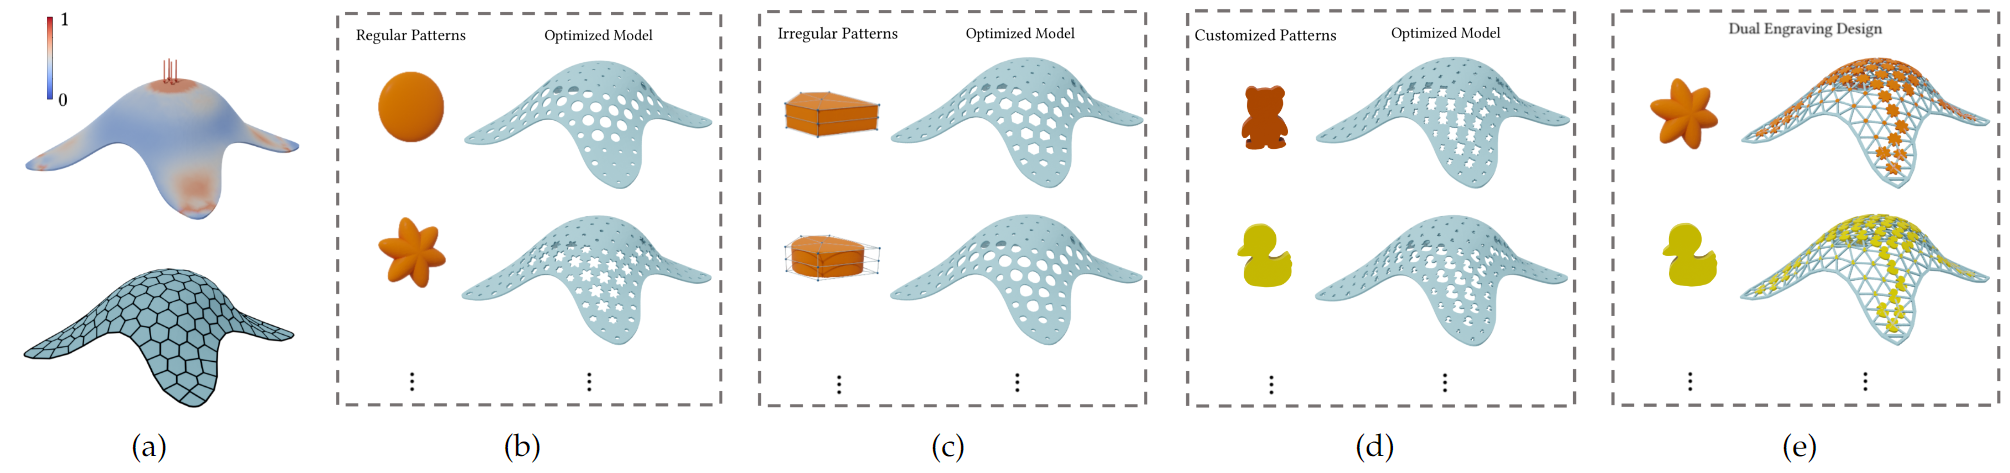
\includegraphics[width=1.0\linewidth]{./figures/thin-shell-1}
    \caption{基于隐式表示的                              薄壳(对偶)雕刻设计优化方法}
    \label{fig:thin-shell-1}
\end{figure}

\section{研究方法}

本方法基于结构的隐式表示设计了一种用于薄壳结构雕刻设计的参数化方法,算法流程如图~\ref{fig:thin-shell-pipeline} 所示。首先,使用函数表示构建三种类型的图案模板,包括规则图案、不规则图案和用户指定的个性化图案。这些图案模板具有可调整的属性, 例如位置、方向和大小, 可以通过参数控制(第~\ref{subsec:parametric-design}节)。然后,将这些模板图案用于壳体结构的雕刻。由于使用有向距离场(SDF)表示输入壳体,因此可以在图案模板和壳体模型之间执行函数布尔运算。最后,为了确保雕刻壳体结构的完整性,引入了结构力学问题的优化模型。以最小应变能为目标,给定体积为约束,该框架可以根据结构响应分析优化图案的属性变量。优化后的(对偶)雕刻壳体结构可以简单地用函数的零等值面表示(第~\ref{}节)。在各种壳体模型上成功实现了该算法,并进行了多组实验,验证了该框架的有效性和鲁棒性(第~\ref{}节)。


\begin{figure}[htbp]
    \centering
    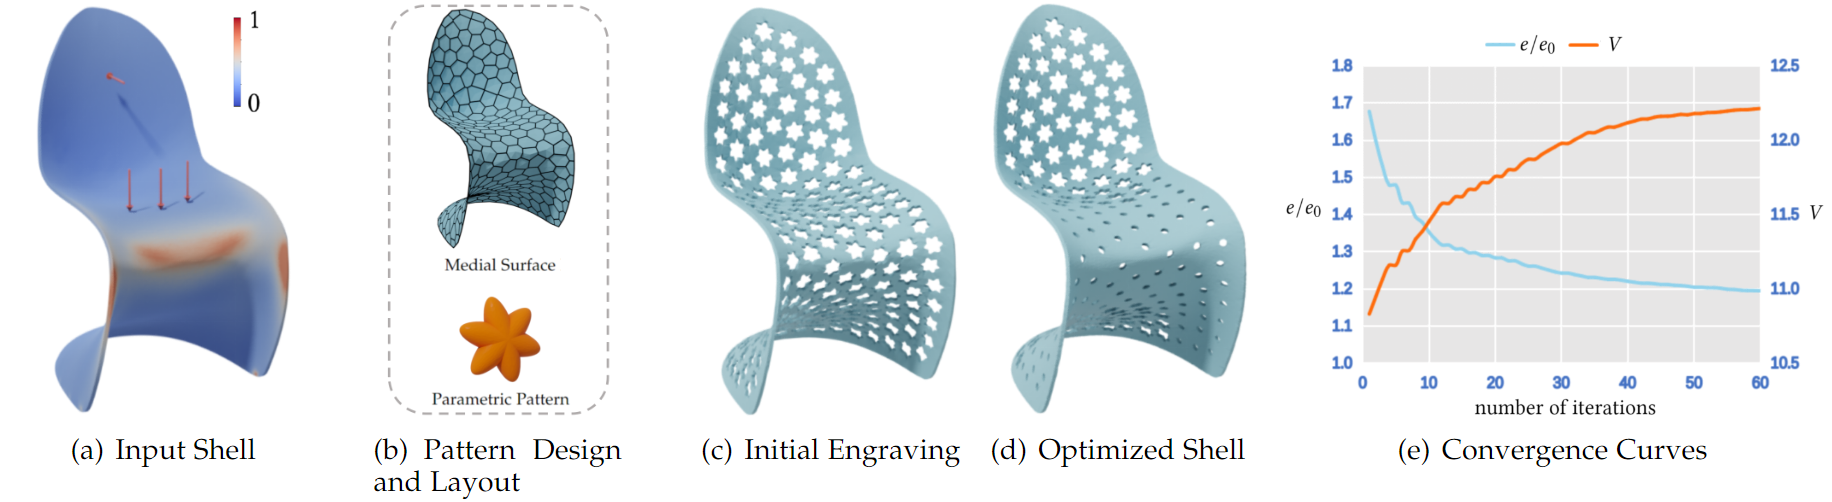
\includegraphics[width=1.0\linewidth]{./figures/thin-shell-pipeline}
    \caption{薄壳雕刻设计方法流程图}
    \label{fig:thin-shell-pipeline}
\end{figure}


\subsection{参数化设计}
\label{subsec:parametric-design}
本文算法采用隐式函数来表示输入模型和图案模板,从而将复杂的结构优化转化为可控参数设计问题,如此便可以高效、鲁棒和可扩展的方式进行结构的设计和优化。

\subsubsection{图案模板设计}
本文提出了三种用于薄壳结构雕刻设计的图案模板类型,包括规则图案、非规则图案和个性化图案,所有这些图案都可以用隐式函数表示。

\paragraph{规则图案。}首先考虑旋转对称的规则图案,并使用超椭球方程构造它们,
\begin{equation}
    \label{eq-ellipsoid}
    E(\mathbf{r})=\left(\frac{\hat{x}}{L_1}\right)^p+\left(\frac{\hat{y}}{L_2}\right)^p+\left(\frac{\hat{z}}{L_3}\right)^p-1,
\end{equation}
其中 $\mathbf{r}=(x, y, z)^\top\in\Omega$ 为三维空间 $\mathbb{R}^3$ 中的设计域,  $\mathbf{c}_0=(x_0,y_0,z_0)^\top$ 是超椭球的中心坐标。
定义 $\hat{\mathbf{r}}=(\hat{x}, \hat{y}, \hat{z})^\top=\mathbf{R}(\mathbf{r}-\mathbf{c}_0)$, 其中 $\mathbf{R}=\{R_{ij}\}_{3\times 3}$ 为旋转矩阵用于调整超椭球的方向。 $L_1$,$L_2$,和 $L_3$ 是超椭球的三个轴长,$p$ 是形状因子,是一个大于零的偶数。当 $p$ 增大时,超椭球逼近一个长方体。

通过控制少量参数,多个超椭球可以构成丰富复杂的图案结构。可以在局部坐标系中围绕其中心点旋转一个超椭球,以获得新的图案, 如图~\ref{fig-ellip} 所示。Specifically, assuming that a pattern is composed of $n$ super-ellipsoids $\{E_i\}_{i=1}^n$, the rotation angle of the $k$-$th$ super-ellipsoid should be $\frac{k\pi}{n}$, $k=1,2,\cdots,n$. 
We compute the orientation of super-ellipsoid $E_k$ by the rotation matrix $\Lambda(\frac{k\pi}{n})\mathbf{R}$, where $\Lambda(\theta)$ is the $z$-axis rotation matrix 